% Holodecks template version of 2023-09-01 enhances the ACM template, version 1.7.0:
% https://www.acm.org/publications/proceedings-template
% The ACM Latex guide provides further information about the ACM template

\documentclass[sigconf, nonacm]{acmart}

%% The following content must be adapted for the final version
% paper-specific
\newcommand\holodoi{XX.XX/XXX.XX}
\newcommand\holopages{XXX-XXX}
% issue-specific
\newcommand\holovolume{1}
\newcommand\holoissue{1}
\newcommand\holoyear{2023}
% should be fine as it is
\newcommand\holoauthors{\authors}
\newcommand\holotitle{\shorttitle} 
% leave empty if no availability url should be set
\newcommand\holoavailabilityurl{URL_TO_YOUR_ARTIFACTS}
% whether page numbers should be shown or not, use 'plain' for review versions, 'empty' for camera ready
\newcommand\holopagestyle{plain} 

\begin{document}
\title{Konzeption eines Projektmanagement Task-Boards unter Anwendung des Habitica Gamification-Ansatzes}

%%
%% The "author" command and its associated commands are used to define the authors and their affiliations.
\author{Nick Philipp Häcker}
\affiliation{%
  \institution{Fakultät für Digitale Medien}
  \institution{Hochschule Furtwangen University}
}
\email{nick.athaeck@gmail.com}




%%
%% The abstract is a short summary of the work to be presented in the
%% article.
\begin{abstract}
% What is a Holodeck?  ChatGPT said ``A holodeck, short for "holographic deck," is a fictional technology that appears in the Star Trek science fiction franchise. It is a key feature on starships and space stations in the Star Trek universe, particularly on Federation starships. The holodeck is a highly advanced and immersive virtual reality environment that uses a combination of holographic projectors, force fields, replicators, and other advanced technologies to create highly realistic and interactive simulations.

% Within a holodeck, users can experience a wide range of environments, scenarios, and adventures. They can interact with computer-generated characters, objects, and settings as if they were real. The holodeck can be used for training, recreation, scientific research, and entertainment. It is often used by the crew of starships to relax, exercise, or engage in historical and adventure simulations.

% The concept of the holodeck has captured the imagination of many Star Trek fans and has inspired discussions and speculation about the feasibility of creating such immersive virtual environments in real life, although, as of my last knowledge update in January 2022, we are still far from achieving the level of technology depicted in the Star Trek series.  An ACM Multimedia Asia 2021 article describes the technology."  That would be~\cite{shahram2021,shahram2022}.
\end{abstract}

\maketitle

%%% do not modify the following Holodeck block %%
%%% Holodeck block start %%%
\pagestyle{\holopagestyle}
\begingroup\small\noindent\raggedright\textbf{CCS Concepts:}\\
% \holoauthors. \holotitle. Holodecks, \holovolume(\holoissue): \holopages, \holoyear.\\
% \href{https://doi.org/\holodoi}{doi:\holodoi}
\endgroup
\begingroup
% \renewcommand\thefootnote{}\footnote{\noindent
% This work is licensed under the Creative Commons BY-NC-ND 4.0 International License. Visit \url{https://creativecommons.org/licenses/by-nc-nd/4.0/} to view a copy of this license. For any use beyond those covered by this license, obtain permission by emailing \href{mailto:info@holodecks.quest}{info@holodecks.quest}. Copyright is held by the owner/author(s). Publication rights licensed to the Holodecks Foundation. \\
% \raggedright Proceedings of the Holodecks Foundation, Vol. \holovolume, No. \holoissue\ %
% ISSN XXXX-XXXX. \\
% \href{https://doi.org/\holodoi}{doi:\holodoi} \\
% }\addtocounter{footnote}{-1}\endgroup
%%% Holodecks block end %%%

%%% do not modify the following Holodecks block %%
%%% Holodecks block start %%%
\ifdefempty{\holoavailabilityurl}{}{
\vspace{.3cm}
\begingroup\small\noindent\raggedright\textbf{Keywords}\\
% The source code, data, and/or other artifacts have been made available at \url{\holoavailabilityurl}.
\endgroup
}
%%% Holodecks block end %%%

\section{Einleitung}

% What is good research?  ChatGPT said "Good research refers to a systematic and rigorous process of investigation aimed at generating new knowledge, solving problems, or contributing to the understanding of a particular subject. Whether in the fields of science, social sciences, humanities, or any other discipline, good research typically exhibits the following key characteristics:"

\subsection{Aufbau des Papers}

\section{Stand der Forschung}

\subsection{Gamification}

\subsection{Projektmanagement Tools}

\section{Ansatz der Konzeption}

\subsection{Analyse von Habitica}

\subsection{Analyse von Asana}

\section{Fazit und Ausblick}
% A scientific manuscript is a formal document that presents the results of scientific research for publication in a scholarly journal or for sharing with the scientific community. While the specific requirements and formatting may vary by journal and field of study, there are some core structural components that are typically found in most scientific manuscripts. These components help organize and present the research in a clear and standardized way. 

% \subsection{Figures}

% Scientific figures are visual representations of data, information, or concepts that are used to illustrate and convey key findings, relationships, and details in a scientific context. These figures play a crucial role in scientific research and communication, helping researchers and readers understand complex data and concepts more effectively.   See Figure~\ref{fig:haptic}.

% \begin{figure}
%   \centering
%   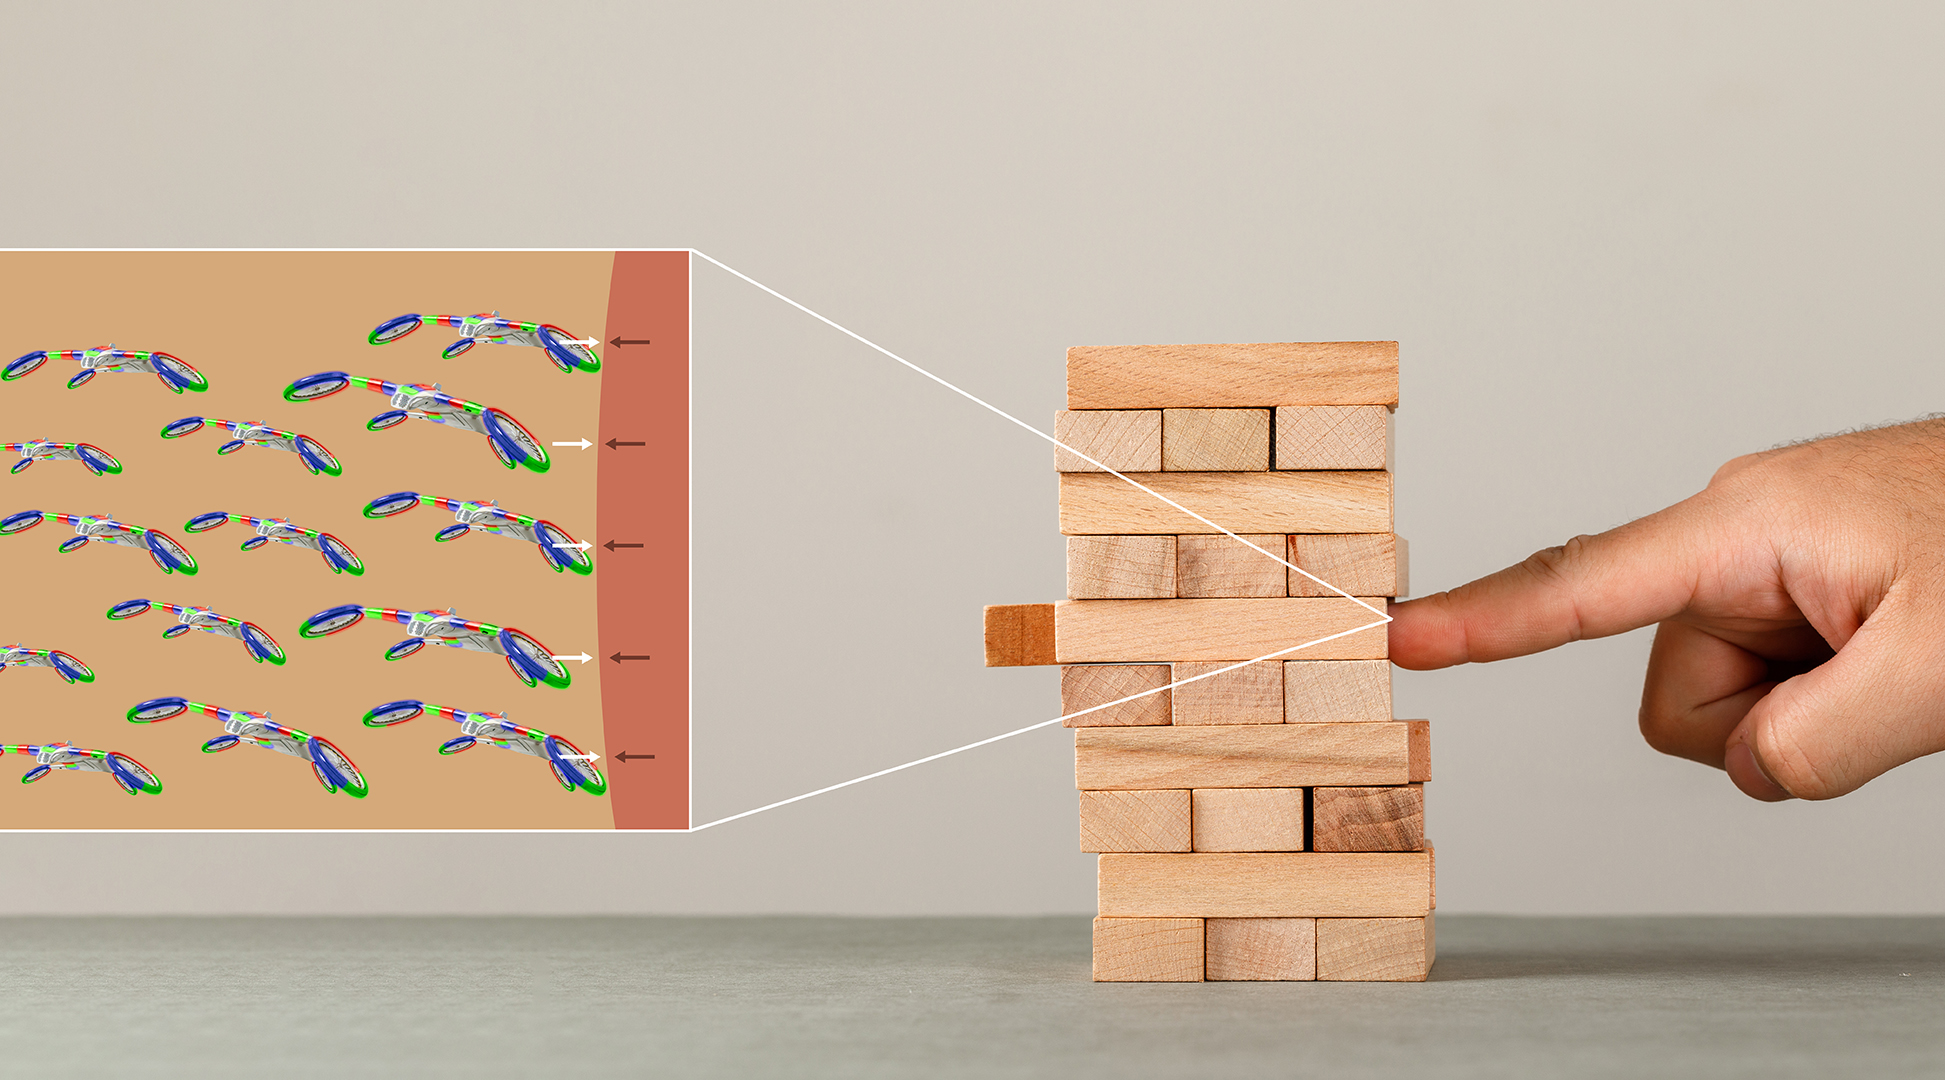
\includegraphics[width=\linewidth]{push_1.jpg}
%   \caption{An illustration of haptic interaction in a Holodeck.}
%   \label{fig:haptic}
% \end{figure}

% \begin{table*}[t]
%   \caption{A double column table.}
%   \label{tab:commands}
%   \begin{tabular}{ccl}
%     \toprule
%     A Wide Command Column & A Random Number & Comments\\
%     \midrule
%     \verb|\tabular| & 100& The content of a table \\
%     \verb|\table|  & 300 & For floating tables within a single column\\
%     \verb|\table*| & 400 & For wider floating tables that span two columns\\
%     \bottomrule
%   \end{tabular}
% \end{table*}

% \subsection{Tables}

% Scientific tables are organized grids or matrices used to present structured and tabular data in a clear and systematic manner in scientific publications. These tables are commonly used in research papers, reports, articles, and other scientific documents to present numerical or categorical data, comparisons, and detailed information that may be difficult to convey effectively in the text. Scientific tables help readers quickly grasp and reference key data without the need for extensive prose. See \autoref{tab:commands}.

% Data should be collected carefully and analyzed using appropriate tools and techniques. The analysis should be objective and unbiased. \autoref{tab:freq}. 

% \begin{table}[hb]% h asks to places the floating element [h]ere.
%   \caption{Frequency of Special Characters}
%   \label{tab:freq}
%   \begin{tabular}{ccl}
%     \toprule
%     Non-English or Math & Frequency & Comments\\
%     \midrule
%     \O & 1 in 1000& For Swedish names\\
%     $\pi$ & 1 in 5 & Common in math\\
%     \$ & 4 in 5 & Used in business\\
%     $\Psi^2_1$ & 1 in 40\,000 & Unexplained usage\\
%   \bottomrule
% \end{tabular}
% \end{table}

% Scientific tables are used to present a wide range of data, including experimental results, survey data, statistical analyses, and any information that can be organized in a tabular format.

% \subsection{Listings and Styles}

% Researchers must adhere to ethical guidelines, ensuring that the rights and well-being of participants are protected, and that the research is conducted with integrity.

% \begin{itemize}
% \item Clarity and Transparency: The research should be presented in a clear and transparent manner. This includes providing details about the methodology, data sources, and any potential conflicts of interest.
% \item Contribution to Knowledge: Good research should make a meaningful contribution to the existing body of knowledge in its field. It should advance understanding, provide insights, or offer practical solutions to problems.
% \item Peer Review: Research is often subject to peer review by experts in the field. Passing peer review is an indicator of the quality and credibility of the research.
% \end{itemize}

% Good research requires attention to detail, critical thinking, and a commitment to following best practices in the field. It contributes to the advancement of knowledge and often forms the basis for further studies and innovations.

% \begin{enumerate}
% \item Reproducibility: Ideally, research findings should be reproducible by other researchers following the same methodology. This ensures the robustness of the results.
% \item Impact: Depending on the field and research objectives, good research may have a real-world impact, such as informing policy decisions, improving technologies, or enhancing our understanding of the world.
% \item Effective Communication: The results of research should be communicated effectively through publications, presentations, or other means so that they can be understood and utilized by the broader community.
% \end{enumerate}

% Science is a broad and diverse field, encompassing various disciplines such as physics, chemistry, biology, astronomy, geology, psychology, sociology, and many more. Each discipline uses the scientific method and principles to explore specific aspects of the natural world and answer questions related to their respective domains.

% \subsection{Math and Equations}

% Mathematics, often simply referred to as "math," is a fundamental field of study that deals with numbers, quantities, structures, patterns, and relationships. It is a universal language and a powerful tool for understanding and describing the world around us. Mathematics provides a systematic way to analyze, solve problems, and make predictions.
% \begin{equation}
%   \lim_{n\rightarrow \infty}x=0
% \end{equation}

% Calculus is concerned with rates of change and accumulation. It includes differential calculus, which deals with derivatives and slopes, and integral calculus, which deals with areas and accumulation. 
% \begin{displaymath}
%   \sum_{i=0}^{\infty} x + 1
% \end{displaymath}

% Mathematics is not just a subject of study but also a powerful tool used in various fields, including physics, engineering, computer science, economics, and the natural and social sciences. It underlies many technological advancements and scientific discoveries. 
% \begin{equation}
%   \sum_{i=0}^{\infty}x_i=\int_{0}^{\pi+2} f
% \end{equation}

% Mathematics is often considered the "language of science" because it provides a precise and unambiguous means of expressing and communicating complex ideas and relationships. It is an integral part of our daily lives and is used in a wide range of practical applications, from budgeting and financial analysis to designing algorithms and understanding the fundamental laws of the universe.

% \section{Citations}

% Some examples of references. A paginated journal article~\cite{Abril07}, an enumerated journal article~\cite{Cohen07}, a reference to an entire issue~\cite{JCohen96}, a monograph (whole book) ~\cite{Kosiur01}, a monograph/whole book in a series (see 2a in spec. document)~\cite{Harel79}, a divisible-book such as an anthology or compilation~\cite{Editor00} followed by the same example, however we only output the series if the volume number is given~\cite{Editor00a} (so Editor00a's series should NOT be present since it has no vol. no.), a chapter in a divisible book~\cite{Spector90}, a chapter in a divisible book in a series~\cite{Douglass98}, a multi-volume work as book~\cite{Knuth97}, an article in a proceedings (of a conference, symposium, workshop for example) (paginated proceedings article)~\cite{Andler79}, a proceedings article with all possible elements~\cite{Smith10}, an example of an enumerated proceedings article~\cite{VanGundy07}, an informally published work~\cite{Harel78}, a doctoral dissertation~\cite{Clarkson85}, a master's thesis~\cite{anisi03}, an finally two online documents or world wide web resources~\cite{Thornburg01, Ablamowicz07}.

% \balance

% \begin{acks}
%  This work was supported by the [...] Research Fund of [...] (Number [...]). Additional funding was provided by [...] and [...]. We also thank [...] for contributing [...].
% \end{acks}

%\clearpage

\bibliographystyle{ACM-Reference-Format}
\bibliography{sample}

\end{document}
\endinput
